\hypertarget{ux57faux4e8eux9690ux53d8ux91cfux9884ux6d4bux652fux6301ux4e0bux6e38ux4efbux52a1ux7684ux4e16ux754cux6a21ux578b}{%
\chapter{基于隐变量预测支持下游任务的世界模型}\label{ux57faux4e8eux9690ux53d8ux91cfux9884ux6d4bux652fux6301ux4e0bux6e38ux4efbux52a1ux7684ux4e16ux754cux6a21ux578b}}

\hypertarget{rlux4e2dux7684ux4e16ux754cux6a21ux578b}{%
\section{RL中的世界模型}\label{rlux4e2dux7684ux4e16ux754cux6a21ux578b}}

\hypertarget{ux4e00ux6838ux5fc3ux601dux60f3-23}{%
\subsection{一、核心思想}\label{ux4e00ux6838ux5fc3ux601dux60f3-23}}

人类在感知世界时，会根据自身有限的感官信息在脑海中建立对世界的心理模型。我们做出的决定和行动正是基于这个内部模型。受此认知科学理念的启发，本文探讨了为强化学习（RL）环境构建生成式神经网络模型。

研究者将智能体划分为世界模型和控制模型。世界模型学习环境在空间和时间上的压缩表示；控制模型利用从世界模型中提取的特征作为输入，训练一个策略来完成任务。

这种方法的优势在于，它不仅能高效处理信度分配（Credit Assignment）问题，还能允许智能体在其世界模型生成的虚拟``梦境''中进行自我训练，然后再将策略迁移到真实环境中，这也就是基于模型的强化学习。

\hypertarget{ux4e8cux6a21ux578bux67b6ux6784ux548cux8badux7ec3ux65b9ux6cd5}{%
\subsection{二、模型架构和训练方法}\label{ux4e8cux6a21ux578bux67b6ux6784ux548cux8badux7ec3ux65b9ux6cd5}}

\hypertarget{ux4e00ux4e16ux754cux6a21ux578b}{%
\subsubsection{（一）世界模型}\label{ux4e00ux4e16ux754cux6a21ux578b}}

\begin{enumerate}
\def\labelenumi{\arabic{enumi}.}
\item
  感知模型：输入t时刻的视觉像素等多模态信息，用变分自编码器（VAE）等将其压缩成一个小型的向量，即隐变量z\_t。
\item
  预测模型：维护隐状态h\_t，运用类似RNN的结构记录历史记忆，以保证长时间内符合物理定律。输入隐状态h\_t、当前状态信息z\_t和动作输出a\_t对未来状态的预测z*\_t+1。可以直接输出采样，或输出未来状态的概率密度函数。根据预测的z*\_t+1和真实下一状态对应的隐变量z\_t+1的差距构造损失函数学习。
\end{enumerate}

\hypertarget{ux4e8cux63a7ux5236ux6a21ux578b}{%
\subsubsection{（二）控制模型}\label{ux4e8cux63a7ux5236ux6a21ux578b}}

控制模型即被通过强化学习训练的策略网络、价值网络等。一般和世界模型有三种协同方法：

\begin{enumerate}
\def\labelenumi{\arabic{enumi}.}
\item
  控制模型的输入不包括世界模型的输出，但在对控制模型输出进行组采样等的时候，结合世界模型的输出。
\item
  将世界模型的输出一并输入控制模型。
\item
  将二者直接合一，保留多头输出。
\end{enumerate}

\hypertarget{ux4e09ux8badux7ec3ux5de5ux4f5cux6d41-3}{%
\subsection{三、训练工作流}\label{ux4e09ux8badux7ec3ux5de5ux4f5cux6d41-3}}

训练的过程是以下步骤的循环：

\begin{enumerate}
\def\labelenumi{\arabic{enumi}.}
\item
  冻结模型权重，智能体与真实环境互动，收集状态-动作对数据。
\item
  运用数据训练感知模型。
\item
  再冻结感知模型，训练预测模型。
\item
  最后冻结感知模型和预测模型，训练控制模型。
\end{enumerate}

\hypertarget{ux56dbux5bf9ux6297ux6027ux7b56ux7565}{%
\subsection{四、对抗性策略}\label{ux56dbux5bf9ux6297ux6027ux7b56ux7565}}

由于世界模型只是对真实环境的近似概率模型，控制器在优化过程中可能会发现并利用这些不完美的漏洞，产生``对抗性策略''（例如以一种特定的移动方式让生成的火球凭空熄灭）。适当提高预测模型的温度参数来增加虚拟环境的不确定性和随机性，可以有效防止控制器利用这些模型缺陷。这使得智能体学会了更稳健的策略，从而在真实环境中的表现更好。

\hypertarget{ux53c2ux8003ux6587ux732e-186}{%
\subsection{参考文献}\label{ux53c2ux8003ux6587ux732e-186}}

\begin{itemize}
\tightlist
\item
  Ha, D., \& Schmidhuber, J. (2018). \href{https://arxiv.org/abs/1803.10122}{World Models}. arXiv:1803.10122.
\item
  Hafner, D., Lillicrap, T., Fischer, I., et al.~(2019). \href{https://arxiv.org/abs/1811.04551}{Learning Latent Dynamics for Planning from Pixels}. ICML.
\item
  Hafner, D., Pasukonis, J., Ba, J., \& Lillicrap, T. (2023). \href{https://arxiv.org/abs/2301.04104}{Mastering Diverse Domains through World Models}. arXiv:2301.04104.
\end{itemize}

\clearpage

\hypertarget{rssmux4e0eblock-causal-transformer}{%
\section{RSSM与Block-Causal Transformer}\label{rssmux4e0eblock-causal-transformer}}

\hypertarget{ux4e00rssm}{%
\subsection{一、RSSM}\label{ux4e00rssm}}

\hypertarget{ux4e00ux6a21ux578bux67b6ux6784}{%
\subsubsection{（一）模型架构}\label{ux4e00ux6a21ux578bux67b6ux6784}}

在构建环境动力学模型时，通常有两种极端：

\begin{enumerate}
\def\labelenumi{\arabic{enumi}.}
\item
  \textbf{纯确定性模型（如标准 RNN）}：状态转移是完全确定的。这种模型容易出现的一个致命缺陷是，它无法捕捉环境动力学中固有的不确定性和多种可能的未来（Multiple futures）。如果用于规划，规划器（Planner）会很容易利用这种确定性模型的不准确性（即过拟合到单一的错误未来）。
\item
  \textbf{纯随机性模型（如传统 SSM）}：每一次状态转移都包含从概率分布中采样。虽然这能建模不确定性，但纯粹的随机转换使得模型极难在跨越多个时间步的情况下可靠地记忆信息。
\end{enumerate}

而且，如果环境存在随机性，确定性网络往往会输出所有可能未来的``模糊平均值''。

RSSM采用了类似LSTM的方法，将隐状态（历史记忆）和反映当前状态的潜变量分开，从而结合了二者的优点。在POMDP（部分可观测马尔可夫决策过程）中：

历史记忆 \(h_t\) 作为隐状态，其转移用确定性规则：由 \(t-2\) 时刻及以前的记忆 \(h_{t-1}\)、\(t-1\) 时刻的状态潜变量 \(s_{t-1}\) 和 \(t-1\) 时刻的动作 \(a_{t-1}\) 经过函数得到。

\begin{enumerate}
\def\labelenumi{\arabic{enumi}.}
\tightlist
\item
  \textbf{确定性状态模型（Deterministic state model）}
\end{enumerate}

\[
h_t = f(h_{t-1}, s_{t-1}, a_{t-1})
\]

\begin{itemize}
\tightlist
\item
  \textbf{物理意义}：用于汇总历史信息并维持跨越多个时间步的确定性记忆。
\item
  \textbf{拟合方式}：通常由一个循环神经网络（RNN，如 GRU）拟合。
\end{itemize}

利用包含 \(t-1\) 时刻及以前状态和动作的历史记忆 \(h_t\) 预测世界状态潜变量 \(s_t\)，则随机采样：

\begin{enumerate}
\def\labelenumi{\arabic{enumi}.}
\setcounter{enumi}{1}
\tightlist
\item
  \textbf{随机状态模型 / 先验分布（Stochastic state model / Prior）}
\end{enumerate}

\[
s_t \sim p(s_t \mid h_t)
\]

\begin{itemize}
\tightlist
\item
  \textbf{物理意义}：在不观察当前真实图像的情况下，仅凭过去的记忆预测当前可能的状态分布。它为模型引入了不确定性，以刻画多种可能的未来。
\item
  \textbf{拟合方式}：由一个多层感知机（MLP）拟合，输出对角高斯分布的均值和方差。
\end{itemize}

而实际上世界状态的潜变量 \(s_t\)（也就是获得当前真实观测 \(o_t\) 后的``预测正确答案''）：（注：理论上可用贝叶斯计算，但涉及不可求的积分，故直接用神经网络拟合）

\begin{enumerate}
\def\labelenumi{\arabic{enumi}.}
\setcounter{enumi}{2}
\tightlist
\item
  \textbf{近似后验模型 / 变分编码器（Approximate posterior / Variational Encoder）}
\end{enumerate}

\[
q(s_t \mid h_t, o_t)
\]

\begin{itemize}
\tightlist
\item
  \textbf{物理意义}：结合过去的确定性记忆 \(h_t\) 和当前的真实高维像素观测 \(o_t\)，推断出当前最准确的潜在状态分布。
\item
  \textbf{拟合方式}：由卷积神经网络（CNN）提取图像特征后，接多层感知机（MLP）输出对角高斯分布的均值和方差。
\end{itemize}

当我们预测出 \(s_t\) 后，可基于 \(h_t\) 和 \(s_t\) 生成像素图像 \(o_t\)：

\begin{enumerate}
\def\labelenumi{\arabic{enumi}.}
\setcounter{enumi}{3}
\tightlist
\item
  \textbf{观测重构模型（Observation model / Decoder）}
\end{enumerate}

\[
o_t \sim p(o_t \mid h_t, s_t)
\]

\begin{itemize}
\tightlist
\item
  \textbf{物理意义}：验证潜在状态是否包含了足够的环境信息，通过潜在状态还原出高维的像素图像。
\item
  \textbf{拟合方式}：由反卷积神经网络（Deconvolutional Neural Network）拟合。
\end{itemize}

以及预测奖励：

\begin{enumerate}
\def\labelenumi{\arabic{enumi}.}
\setcounter{enumi}{4}
\tightlist
\item
  \textbf{奖励预测模型（Reward model）}
\end{enumerate}

\[
r_t \sim p(r_t \mid h_t, s_t)
\]

\begin{itemize}
\tightlist
\item
  \textbf{物理意义}：预测在当前潜在状态下能获得的标量奖励，这是规划器（Planner）在潜在空间中评估动作好坏的唯一依据。
\item
  \textbf{拟合方式}：由多层感知机（MLP）拟合。
\end{itemize}

\hypertarget{ux4e8cux5de5ux4f5cux6d41-9}{%
\subsubsection{（二）工作流}\label{ux4e8cux5de5ux4f5cux6d41-9}}

\begin{itemize}
\tightlist
\item
  \textbf{步骤 1：数据采样}
\end{itemize}

从经验回放池 \(\mathcal{D}\) 中均匀随机抽取批量大小为 \(B\)、长度为 \(L\) 的序列片段 \(\{(o_t, a_t, r_t)_{t=k}^{L+k}\}_{i=1}^{B}\)。

\begin{itemize}
\tightlist
\item
  \textbf{步骤 2：状态展开与分布计算（Forward Pass）}
\end{itemize}

对于序列中的每一个时间步 \(t = 1 \ldots L\)：

\begin{enumerate}
\def\labelenumi{\arabic{enumi}.}
\tightlist
\item
  执行确定性状态转移：将上一步的 \(h_{t-1}\)、\(s_{t-1}\)（通过重参数化采样得到）和动作 \(a_{t-1}\) 输入 RNN \(f\)，得到当前的确定性状态 \(h_t\)。
\item
  计算先验分布 \(p\)：将 \(h_t\) 输入 MLP，输出当前先验高斯的均值和方差 \(\mu_{\mathrm{prior}}\)、\(\sigma_{\mathrm{prior}}\)。
\item
  计算后验分布 \(q\)：将当前的图像 \(o_t\) 通过 CNN 提取特征，结合 \(h_t\) 输入到另一个 MLP，输出后验高斯的均值和方差 \(\mu_{\mathrm{post}}\)、\(\sigma_{\mathrm{post}}\)。
\item
  重参数化采样：从后验分布 \(\mathcal{N}(\mu_{\mathrm{post}}, \sigma_{\mathrm{post}}^2)\) 中采样出潜在向量 \(s_t\)。
\end{enumerate}

\begin{itemize}
\tightlist
\item
  \textbf{步骤 3：计算重构与预测}
\end{itemize}

将 \(h_t\) 和采样得到的 \(s_t\) 输入反卷积解码器预测重构图像 \(\hat{o}_t\)，并输入奖励模型预测标量奖励 \(\hat{r}_t\)。

\begin{itemize}
\tightlist
\item
  \textbf{步骤 4：损失计算（Loss Computation）}
\end{itemize}

\begin{enumerate}
\def\labelenumi{\arabic{enumi}.}
\tightlist
\item
  计算重构图像 \(\hat{o}_t\) 与真实图像 \(o_t\) 的 MSE（重构损失）。
\item
  计算预测奖励 \(\hat{r}_t\) 与真实奖励 \(r_t\) 的 MSE。
\item
  计算先验分布 \(p\) 与后验分布 \(q\) 之间的 KL 散度（如果使用 Latent Overshooting，还需要并行计算并累加跨越多步的先验与当前后验的 KL 散度）。
\end{enumerate}

\begin{itemize}
\tightlist
\item
  \textbf{步骤 5：参数更新（Backpropagation）}
\end{itemize}

将所有时间步的损失累加求平均得到总损失 \(\mathcal{L}(\theta)\)，使用优化器（如 Adam）计算梯度，更新构成这 5 个函数的所有神经网络参数 \(\theta \leftarrow \theta - \alpha \nabla_{\theta}\mathcal{L}(\theta)\)。

\hypertarget{ux4e09ux635fux5931ux51fdux6570-3}{%
\subsubsection{（三）损失函数}\label{ux4e09ux635fux5931ux51fdux6570-3}}

损失分为三部分：仅有过去记忆时对现在潜变量的预测p和包含过去记忆与现在观测时的真实现在潜变量q之间的KL散度，体现的是预测下一时刻的潜变量和真实下一时刻的潜变量的差距，反映预测下一时刻状态的能力；图像重构损失反映由潜变量重构像素的能力；奖励损失反映由潜变量预测奖励的能力。表达式如下：

\[
\begin{aligned}
\mathcal{L}
&=
\sum_{t=1}^{T}
\Biggl(
-\mathbb{E}_{q(s_t \mid o_{\le t}, a_{<t})}
\left[\ln p(o_t \mid s_t) + \ln p(r_t \mid s_t)\right]
\\
&\quad+
\mathbb{E}
\left[
D_{\mathrm{KL}}\left(
q(s_t \mid o_{\le t}, a_{<t})
\parallel
p(s_t \mid s_{t-1}, a_{t-1})
\right)
\right]
\Biggr)
\end{aligned}
\]

这里 \(o_t\) 和 \(r_t\) 均满足高斯分布，故这两项等价于 MSE Loss。

由于标准目标只通过一步 KL 散度训练随机路径，模型在多步预测时容易发散。Latent Overshooting 将约束扩展到距离为 \(d\) 的所有未来时间步：

\[
\begin{aligned}
\mathcal{L}_{\mathrm{overshooting}}(\theta)
&=
\sum_{t=1}^{T}
\Biggl(
-\mathbb{E}_{q}\left[\ln p(o_t \mid s_t)\right]
\\
&\quad+
\frac{1}{D}
\sum_{d=1}^{D}
\beta_d
\mathbb{E}
\left[
D_{\mathrm{KL}}\left(
q(s_t \mid o_{\le t})
\parallel
p(s_t \mid s_{t-d})
\right)
\right]
\Biggr)
\end{aligned}
\]

\begin{itemize}
\tightlist
\item
  \textbf{物理意义}：它不仅要求``由 \(t - 1\) 步预测的 \(t\) 步先验''要与后验对齐，还要求``由 \(t - 2\) 步、\(t - d\) 步连续多步推演得出的 \(t\) 步先验''也要与当前后验对齐。这种潜在空间中的一致性正则化，增强了模型在不依赖真实观测时的长期演化能力。
\end{itemize}

\hypertarget{ux4e8cux57faux4e8erssmux7684ux5e94ux7528}{%
\subsection{二、基于RSSM的应用}\label{ux4e8cux57faux4e8erssmux7684ux5e94ux7528}}

\hypertarget{ux4e00planetux57faux4e8eux4e16ux754cux6a21ux578bux7684ux641cux7d22ux89c4ux5212}{%
\subsubsection{（一）PlaNet：基于世界模型的搜索规划}\label{ux4e00planetux57faux4e8eux4e16ux754cux6a21ux578bux7684ux641cux7d22ux89c4ux5212}}

\begin{enumerate}
\def\labelenumi{\arabic{enumi}.}
\tightlist
\item
  \textbf{外层循环：模型训练与数据收集（Algorithm 1）}
\end{enumerate}

\begin{itemize}
\tightlist
\item
  \textbf{初始化}：使用随机动作收集少量初始种子回合（Seed episodes），存入经验回放池 \(\mathcal{D}\)。
\item
  \textbf{模型拟合}：从 \(\mathcal{D}\) 中随机抽取数据块，利用上述变分下界公式计算损失，并通过梯度上升更新 RSSM 的参数 \(\theta\)。
\item
  \textbf{环境交互}：使用更新后的模型，通过规划算法（见下文 CEM）选择动作 \(a_t\)，在动作上加入高斯探索噪声，与环境交互并将新经验存入 \(\mathcal{D}\)。
\end{itemize}

\begin{enumerate}
\def\labelenumi{\arabic{enumi}.}
\setcounter{enumi}{1}
\tightlist
\item
  \textbf{内层循环：基于 CEM 的动作规划（Algorithm 2）}
\end{enumerate}

在每一个时间步，智能体不使用策略网络（Policy Network）输出动作，而是通过交叉熵方法（Cross Entropy Method, CEM）和模型预测控制（MPC）实时搜索最优动作序列：

\begin{itemize}
\tightlist
\item
  \textbf{初始化信念}：构建一个随时间变化的正态分布信念 \(q(a_{t:t+H}) \sim Normal(\mu, \sigma^2 I)\)，用于表示规划视界 \(H\) 内的最佳动作序列。
\item
  \textbf{迭代优化}：

  \begin{enumerate}
  \def\labelenumi{\arabic{enumi}.}
  \tightlist
  \item
    从当前信念中采样 \(J\) 个候选动作序列。
  \item
    将这些序列输入到学习好的 RSSM 模型中，仅在潜在空间中推演未来状态，并计算预期奖励总和 \(R^{(j)}\)。
  \item
    挑选出奖励最高的 \(K\) 个动作序列。
  \item
    使用这 \(K\) 个优秀序列的均值和方差重新拟合动作信念分布。
  \end{enumerate}
\item
  \textbf{执行与重规划}：经过 \(I\) 次迭代后，提取最终信念均值的第一个动作去执行。由于采用 MPC 机制，接收到新观测后，动作序列的信念会重置为零均值和单位方差，以避免陷入局部最优。
\end{itemize}

\hypertarget{ux4e8cdreamer-3ux5229ux7528ux4e16ux754cux6a21ux578bux8fdbux884crlux8badux7ec3}{%
\subsubsection{（二）Dreamer 3：利用世界模型进行RL训练}\label{ux4e8cdreamer-3ux5229ux7528ux4e16ux754cux6a21ux578bux8fdbux884crlux8badux7ec3}}

\textbf{1. 世界模型}

\begin{itemize}
\tightlist
\item
  世界模型通过自动编码技术，将复杂的感知输入（如图像）压缩成紧凑的潜在表示。
\item
  它被实现为一个循环状态空间模型（RSSM）。
\item
  首先，编码器将感知输入 \(x_t\) 映射为随机表示 \(z_t \sim q_{\phi}(z_t \mid h_t, x_t)\)。
\item
  然后，动力学预测器根据之前的状态 \(h_t\) 预测未来的表示 \(\hat{z}_t \approx p_{\phi}(\hat{z}_t \mid h_t)\)。
\item
  通过这种方式，世界模型学会了理解环境的内在结构，并能在隐空间中``想象''未来的状态演变。
\end{itemize}

在数学上，RSSM 是一种结合了确定性循环神经网络（RNN）和随机状态变量的生成式模型。在时间步 \(t\)，它定义动作 \(a_t\)、观测输入 \(x_t\)、奖励 \(r_t\) 以及回合继续标志 \(c_t \in \{0, 1\}\)。

\textbf{2. Critic}

\textbf{Step 2：评论家学习（Critic Learning）}

\begin{itemize}
\tightlist
\item
  评论家和演员完全在世界模型``想象''出的抽象轨迹中进行学习，而无需直接与真实环境交互。
\item
  评论家接收模型状态 \(s_t = [h_t, z_t]\)，并学习评估该状态的价值。
\item
  为了考虑长期收益，评论家预测的是回报分布的期望值，并使用自举（bootstrapped）的 \(\lambda\)-回报来整合预测的奖励和价值。
\end{itemize}

\textbf{3. Actor}

\textbf{Step 3：演员学习（Actor Learning）}

\begin{itemize}
\tightlist
\item
  演员的目标是选择能够最大化回报的动作，同时通过熵正则化（entropy regularizer）来鼓励探索。
\item
  它通过策略梯度方法（Reinforce estimator）在想象的轨迹上进行优化。
\end{itemize}

\textbf{4. 损失函数}

（1）预测损失

\[
\mathcal{L}_{\mathrm{pred}}(\phi)
\doteq
-\ln p_{\phi}(x_t \mid z_t, h_t)
-\ln p_{\phi}(r_t \mid z_t, h_t)
-\ln p_{\phi}(c_t \mid z_t, h_t)
\]

这部分通过负对数似然，迫使模型准确地重构观测输入、奖励和回合标志。

（2）动力学损失

\[
\mathcal{L}_{\mathrm{dyn}}(\phi)
\doteq
\max\left(
1,
D_{\mathrm{KL}}\left[
\mathrm{sg}(q_{\phi}(z_t \mid h_t, x_t))
\parallel
p_{\phi}(\hat{z}_t \mid h_t)
\right]
\right)
\]

其核心目的是让动力学预测器 \(p_{\phi}\) 逼近编码器给出的后验分布 \(q_{\phi}\)。这里使用 \(\mathrm{sg}(\cdot)\)（stop-gradient，停止梯度）操作，表示在拉近两个分布距离时，只更新动力学预测器的参数，而不影响编码器提取特征的方式。

同时，公式外围包裹的 \(\max(1, \cdot)\) 引入了空闲位（Free bits）技术：当 KL 散度下降到 1 nat \(\approx 1.44\) bits 以下时，模型会停止在这项损失上的惩罚，避免学到过于退化的平凡动力学，从而将学习重点转移回预测损失上。

（3）表示损失

\[
\mathcal{L}_{\mathrm{rep}}(\phi)
\doteq
\max\left(
1,
D_{\mathrm{KL}}\left[
q_{\phi}(z_t \mid h_t, x_t)
\parallel
\mathrm{sg}(p_{\phi}(\hat{z}_t \mid h_t))
\right]
\right)
\]

与上一个损失相反，表示损失的梯度方向被限制在编码器 \(q_{\phi}\) 上。它的目的是反向规范编码器的行为，促使它提取出来的隐状态更加``有规律''、更容易被动力学模型预测。

通过巧妙运用停止梯度操作和不同的损失缩放（在论文中设定为 \(\beta_{\mathrm{pred}} = 1\)、\(\beta_{\mathrm{dyn}} = 1\)、\(\beta_{\mathrm{rep}} = 0.1\)），RSSM 解决了以往``强正则化在简单图像有效，但在复杂 3D 环境会抹杀关键细节''的进退两难问题，实现了跨领域的鲁棒性。

\hypertarget{ux4e09ux7ed3ux5408ux5e76ux884cux626bux63cfux7684ux72b6ux6001ux7a7aux95f4ux6a21ux578b}{%
\subsection{三、结合并行扫描的状态空间模型}\label{ux4e09ux7ed3ux5408ux5e76ux884cux626bux63cfux7684ux72b6ux6001ux7a7aux95f4ux6a21ux578b}}

\hypertarget{ux4e00ux6838ux5fc3ux7b97ux6cd5}{%
\subsubsection{（一）核心算法}\label{ux4e00ux6838ux5fc3ux7b97ux6cd5}}

RSSM 的问题在于，当前时刻的隐状态依赖于上一时刻的输出，且时间步传递中存在非线性激活函数，必须先算 \(t=1\)，再算 \(t=2\)，以此类推，时间复杂度为 \(O(L)\)，成为长轨迹计算的瓶颈。

而S5WM采取如下工作流：

\textbf{步骤 1：收集与采样数据（Data Sampling）}

\begin{itemize}
\tightlist
\item
  从重放缓冲区（Replay Buffer）中均匀采样一批历史序列数据，包含观测 \(o_t\)、动作 \(a_t\)、奖励 \(r_t\) 和连续性标志 \(c_t\)。
\end{itemize}

\textbf{步骤 2：训练状态空间世界模型（World Model Training）}

\begin{itemize}
\tightlist
\item
  \textbf{编码}：编码器（Encoder）将观测图像或状态 \(o_t\) 映射为后验随机表示 \(z_t \sim q_{\phi}(\cdot \mid o_t)\)。
\item
  \textbf{特征融合}：将 \(z_t\) 与上一动作 \(a_t\) 通过多层感知机（MLP）融合为一个输入向量 \(u_t\)。
\item
  \textbf{并行序列建模}：将整个序列的 \(u_{1:L}\) 输入到 S5 块中，利用并行扫描技术一次性并行计算出整个序列的隐藏状态 \(x_{1:L}\) 和确定性表示 \(y_{1:L}\)。
\item
  \textbf{解码与损失计算}：模型使用预测头来预测先验随机状态 \(\hat{z}_t\)、观测 \(\hat{o}_t\)、奖励 \(\hat{r}_t\) 和连续性 \(\hat{c}_t\)。最后通过最小化包含预测损失、动态损失（KL 散度）和表示损失的联合损失函数 \(\mathcal{L}(\phi)\) 来更新世界模型权重。
\end{itemize}

\textbf{步骤 3：训练 Actor-Critic（Actor-Critic Training in Imagination）}

\begin{itemize}
\tightlist
\item
  \textbf{潜在空间想象}：从真实数据中采样初始状态，然后在没有任何环境交互的情况下，利用训练好的世界模型在潜在空间中``想象''出未来视野长度为 \(H\)（如 10 步）的轨迹。
\item
  \textbf{策略更新}：Actor 根据确定性状态 \(y_t\) 和随机状态 \(\hat{z}_t\) 输出动作；Critic 预测引导的 \(\lambda\)-回报（Bootstrapped \(\lambda\)-returns）。利用世界模型的完全可微性，将一阶梯度反向传播给策略网络，从而优化 Actor 和 Critic 的参数。
\end{itemize}

传统的 RSSM 中，后验随机变量 \(z_t\) 的推断不仅依赖于观测 \(o_t\)，还依赖于具有时序依赖的确定性状态 \(y_t\)，即 \(z_t \sim q_{\phi}(\cdot \mid y_t, o_t)\)。这在架构上锁死了并行性。S5WM 的设计中，将后验推断前置解耦：先完全只以当前时刻的观测 \(o_t\) 推断得出，即 \(z_t \sim q_{\phi}(\cdot \mid o_t)\)。这样，所有的 \(z_{1:L}\) 都可以用编码器（CNN）一口气并行计算完毕，随后再送入 S5 序列层进行并行扫描。

线性状态空间模型可写作：

\[
x_t = \bar{A}x_{t-1} + \bar{B}u_t
\]

\[
y_t = Cx_t + Du_t
\]

这里能实现并行的核心在于：

假设将初始元素定义为一个二元组：

\[
e_k = (e_{k,a}, e_{k,b}) := (\bar{A}, \bar{B}u_k)
\]

通过数学推导，序列状态可以展开为一系列二元操作符 \(\bullet\) 的连续运算。这个操作符定义为：

\[
a_i \bullet a_j
=
\left(
a_{j,a} \odot a_{i,a},
a_{j,a} \otimes a_{i,b} + a_{j,b}
\right)
\]

这里 \(\odot\) 代表矩阵乘法，\(\otimes\) 代表矩阵向量乘法。

对于一个长序列的计算，我们不需要像 RNN 那样串行计算：

\[
e_1 \rightarrow (e_1 \bullet e_2) \rightarrow ((e_1 \bullet e_2) \bullet e_3) \cdots
\]

因为满足结合律，可以将其构建成一棵二叉树来并行计算：

\[
(e_1 \bullet e_2) \bullet (e_3 \bullet e_4)
\]

在有足够并行处理器（如 GPU）的情况下，原本 \(O(L)\) 的串行时间复杂度被直接对数化，降维打击至 \(O(\log L)\)。

\hypertarget{ux4e8cux5e76ux884cux72b6ux6001ux91cdux7f6e}{%
\subsubsection{（二）并行状态重置}\label{ux4e8cux5e76ux884cux72b6ux6001ux91cdux7f6e}}

RL中，数据往往由多个回合拼接而成。在不断往回递归的过程中，如果已经到了序列最开始，就需要立即截断，防止上一回合状态污染本回合。

如果在并行计算中遇到截断信号，普通的 SSM 算法会崩溃，因为它不知道如何在并行的树状结构中``清零''。作者扩展了前面的二元操作符，引入连续性预测变量 \(c_k \in \{0, 1\}\)，并将初始元素扩展为三元组：

\[
e_k = (e_{k,a}, e_{k,b}, e_{k,c}) := (\bar{A}, \bar{B}u_k, 1 - c_k)
\]

并设计了带有条件分支的新并行操作符：

\[
a_j \bullet a_i
=
\begin{cases}
(a_{j,a} \odot a_{i,a}, a_{j,a} \otimes a_{i,b} + a_{j,b}, a_{i,c}), & \mathrm{if}\; a_{j,c} = 0 \\
(a_{j,a}, a_{j,b}, a_{j,c}), & \mathrm{if}\; a_{j,c} = 1
\end{cases}
\]

这个分段函数的设计非常关键。当 \(a_{j,c} = 1\) 时（代表回合结束），操作符会直接丢弃来自左侧子树（历史数据）的 \(a_i\) 信息，只保留当前的 \(a_j\) 信息。这就使得模型在执行 \(O(\log L)\) 的大规模并行计算时，能够自动且并行地处理序列中任意位置的``重置''信号。

\hypertarget{ux56dbblock-causal-transformer}{%
\subsection{四、Block-Causal Transformer}\label{ux56dbblock-causal-transformer}}

RSSM作为RNN，在长程规划上存在劣势。Block-Causal Transformer是Transformer在世界模型中的一种应用范式，在Dreamer 4中就用了这种架构。

\textbf{经典因果 Transformer（Standard Causal Transformer）}

它采用严格的 Token 级下三角掩码。对于任意两个 Token 索引 \(i, j \in \{1, 2, \ldots, N\}\)，掩码定义为：

\[
M^{\mathrm{causal}}_{i,j}
=
\begin{cases}
0, & \mathrm{if}\; i \ge j \\
-\infty, & \mathrm{if}\; i \lt j
\end{cases}
\]

这意味着，即使 Token \(i\) 和 Token \(j\) 属于同一帧视频，在序列中排在后面的 Token 也只能单向观测排在前面的 Token。这在自然语言中是合理的，但在图像中会迫使模型采用从左上角到右下角的逐块阅读顺序，破坏同一时刻空间的整体连贯性。

\textbf{Block-Causal Transformer}

它采用块级因果掩码（Block-lower-triangular Mask）。定义映射函数 \(t(i)\) 为 Token \(i\) 所在的时间步（帧序号），其掩码定义为：

\[
M^{\mathrm{block}}_{i,j}
=
\begin{cases}
0, & \mathrm{if}\; t(i) \ge t(j) \\
-\infty, & \mathrm{if}\; t(i) \lt t(j)
\end{cases}
\]

在这个矩阵中，主对角线上是大小为 \(S \times S\) 的全零矩阵块，允许同一时间帧内双向注意力；主对角线右上方则是 \(-\infty\)。当 \(t(i) = t(j)\) 时，也就是两个 Token 在同一时间帧内，\(M^{block}_{i,j} = 0\)。

当用于诸如 Dreamer 4 的交互式动力学建模或物理 PDE 预测时，BCT 的工作流如下：

\begin{enumerate}
\def\labelenumi{\arabic{enumi}.}
\tightlist
\item
  \textbf{数据分块与编码（Tokenization \& Patching）}：将输入的连续视频帧序列离散化，每一帧被切割为 \(S\) 个 Patch，并映射为特征向量序列。
\item
  \textbf{复合位置编码注入（Spatiotemporal Positional Encoding）}：为每个 Token 注入两个维度的位置信息：一个是它在当前帧内的二维空间坐标 \((x, y)\)，另一个是它所在的时间步 \(t\)。
\item
  \textbf{块因果注意力计算（Block-Causal Attention Calculation）}：同帧并行计算时，在第 \(t\) 个 Block 内部，执行 \(S\) 个 Token 的全连接自注意力计算，提取当前帧的高分辨率空间语义和物体关系。历史特征提取时，同帧这 \(S\) 个 Token 共同作为 Query，去 attend 过去所有帧（1 到 \(t - 1\)）生成的 Key 和 Value，捕获时序上的物理动力学。
\item
  \textbf{下一帧块级自回归预测（Block-wise Autoregressive Generation）}：不同于经典 GPT 必须逐个 Token 吐出，BCT 在完成前 \(t\) 帧的上下文建模后，可以直接将其作为上下文先验，向第 \(t + 1\) 帧的完整空间块注入，并行且高效地生成第 \(t + 1\) 帧的完整空间表征。
\end{enumerate}

也就是说，在生成第 \(t+1\) 帧时，它刚开始是噪声向量的组合，前 \(t\) 帧的信息在 Attention 模块中作为上下文不断与之融合。

\hypertarget{ux53c2ux8003ux6587ux732e-187}{%
\subsection{参考文献}\label{ux53c2ux8003ux6587ux732e-187}}

\begin{itemize}
\tightlist
\item
  Hafner, D., Lillicrap, T., Fischer, I., et al.~(2019). \href{https://arxiv.org/abs/1811.04551}{Learning Latent Dynamics for Planning from Pixels}. ICML.
\item
  Hafner, D., Lillicrap, T., Ba, J., \& Norouzi, M. (2020). \href{https://arxiv.org/abs/1912.01603}{Dream to Control: Learning Behaviors by Latent Imagination}. ICLR.
\item
  Hafner, D., Pasukonis, J., Ba, J., \& Lillicrap, T. (2023). \href{https://arxiv.org/abs/2301.04104}{Mastering Diverse Domains through World Models}. arXiv:2301.04104.
\item
  Hafner, D., Yan, W., \& Lillicrap, T. (2025). \href{https://arxiv.org/abs/2509.24527}{Training Agents Inside of Scalable World Models}. arXiv:2509.24527.
\end{itemize}

\clearpage

\hypertarget{ux635fux5931ux5206ux6b65ux89e3ux8026ux8bbaux6587}{%
\section{损失分步解耦（论文）}\label{ux635fux5931ux5206ux6b65ux89e3ux8026ux8bbaux6587}}

\begin{quote}
本文是论文阅读笔记，内容代表对应论文方法或作者理解，不应直接视为领域共识或工程最佳实践。
\end{quote}

\hypertarget{ux4e00ux91cdux5efaux52a8ux529bux5b66ux9884ux6d4bux4e0eux5956ux52b1ux9884ux6d4bux7684ux635fux5931ux89e3ux8026}{%
\subsection{一、重建、动力学预测与奖励预测的损失解耦}\label{ux4e00ux91cdux5efaux52a8ux529bux5b66ux9884ux6d4bux4e0eux5956ux52b1ux9884ux6d4bux7684ux635fux5931ux89e3ux8026}}

损失分步解耦方法是Google DeepMind在世界模型Dreamer 4中的改进。

\hypertarget{ux4e00ux95eeux9898ux80ccux666f-11}{%
\subsubsection{（一）问题背景}\label{ux4e00ux95eeux9898ux80ccux666f-11}}

在 Dreamer 3 中，图像编码器（Encoder）、动力学模型（RSSM）、图像解码器（Decoder）和奖励预测器（Reward Predictor）是作为一个巨大的整体同时训练的。

潜在特征 \(z_t\) 在每一次反向传播时，会同时受到三股力量的拉扯：

\begin{enumerate}
\def\labelenumi{\arabic{enumi}.}
\tightlist
\item
  \textbf{重建梯度（\(\nabla \mathcal{L}_{recp}\)）}：逼着 \(z_t\) 记住画面里的每一片云彩和每一棵树，因为解码器需要重构整个画面。
\item
  \textbf{动力学梯度（\(\nabla \mathcal{L}_{dyn}\)）}：逼着 \(z_t\) 关注物体的运动规律。
\item
  \textbf{奖励预测梯度（\(\nabla \mathcal{L}_{pred}\)）}：逼着 \(z_t\) 把所有注意力都集中在那些能得分的微小物体上，例如远处的怪物或手里的钻石，而忽略暂时没有分数、但对理解物理世界至关重要的背景。
\end{enumerate}

这带来的致命问题是``表征容量的争夺''。当环境非常复杂（如 Minecraft）时，这三股梯度会互相打架。如果奖励信号很强，编码器就会为了迎合奖励预测，而在 \(z_t\) 中丢弃那些``暂时没有奖励，但对理解物理世界至关重要''的背景细节，例如地形起伏。这导致 Dreamer 3 的世界模型在复杂 3D 环境中极易发生表征坍塌。

\hypertarget{ux4e8cux89e3ux8026ux635fux5931ux51fdux6570ux7684ux7ec4ux6210ux90e8ux5206}{%
\subsubsection{（二）解耦损失函数的组成部分}\label{ux4e8cux89e3ux8026ux635fux5931ux51fdux6570ux7684ux7ec4ux6210ux90e8ux5206}}

\begin{enumerate}
\def\labelenumi{\arabic{enumi}.}
\tightlist
\item
  \textbf{Tokenizer 压缩损失}
\end{enumerate}

Dreamer 4 不再像前代那样在潜空间动态推演的同时去重建图像。它首先训练一个 Causal Tokenizer，利用掩码自编码器（MAE, Masked Autoencoder）的逻辑，以 \(p \sim U(0, 0.9)\) 的概率随机遮盖视频块（Patches），只专注于时空特征的极致压缩。

其损失函数抛弃了 Symlog，转而采用纯视觉领域的标准重建与感知损失的组合：

\[
\mathcal{L}_{\mathrm{tokenizer}}
=
\mathrm{MSE}(x, \hat{x})
+
\mathrm{LPIPS}(x, \hat{x})
\]

\begin{itemize}
\tightlist
\item
  MSE 保证像素级别的准确性。
\item
  LPIPS（Learned Perceptual Image Patch Similarity）保证人类视觉感知上的结构完整性，避免生成的特征模糊。
\end{itemize}

\begin{enumerate}
\def\labelenumi{\arabic{enumi}.}
\setcounter{enumi}{1}
\tightlist
\item
  \textbf{动力学预测损失}
\end{enumerate}

这一项即Transformer对下一时刻预测的准确程度。Dreamer 4废弃了Dreamer 3的KL散度，避免在处理长序列时发生模式崩溃，而改用流匹配和Shortcut Forcing方法。

\begin{enumerate}
\def\labelenumi{\arabic{enumi}.}
\setcounter{enumi}{2}
\tightlist
\item
  \textbf{任务与奖励预测损失}
\end{enumerate}

Dreamer 4在世界模型中训练Actor和Critic，世界模型需要输出奖励和动作预测：

在通过海量无标签视频训练好 Tokenizer 和 Dynamics 之后，Dreamer 4 会摄入带标签的数据，例如带有鼠标键盘操作记录的 Minecraft 录像，专门训练一个极其轻量的任务头（Task Head）。这部分损失类似于 Dreamer 3 的 \(\mathcal{L}_{pred}\)，但加入了对具体动作的克隆预测：

\[
\begin{aligned}
\mathcal{L}_{\mathrm{task}}
&=
-
\sum_{n=0}^{L}
\ln p_{\theta}(r_{t+n} \mid h_t)
\\
&\quad -
\sum_{n=0}^{L}
\ln p_{\theta}(a_{t+n} \mid h_t)
\end{aligned}
\]

模型利用 Transformer 聚合出的历史时空上下文 \(h_t\)，同时去最大化未来奖励序列 \(r_{t+n}\) 和真实动作序列 \(a_{t+n}\) 的对数似然。

\hypertarget{ux4e09ux635fux5931ux89e3ux8026ux7684ux597dux5904}{%
\subsubsection{（三）损失解耦的好处}\label{ux4e09ux635fux5931ux89e3ux8026ux7684ux597dux5904}}

\begin{enumerate}
\def\labelenumi{\arabic{enumi}.}
\tightlist
\item
  \textbf{避免梯度冲突}
\end{enumerate}

\begin{itemize}
\tightlist
\item
  \textbf{第一步（视觉独立）}：先只用重建损失（类似 MAE 的自编码器逻辑）把 Tokenizer 训练到极致。此时的 \(z_t\) 是完美的\textbf{纯视觉客观表征}，完全没有被奖励信号污染。训练完后，直接冻结 Tokenizer。
\item
  \textbf{第二步（物理独立）}：在冻结的 Tokenizer 提取的 \(z_t\) 之上，单独训练 Block-Causal Transformer（动力学模型）。此时模型只关心上一帧怎么变成下一帧（Shortcut Forcing），完全不知道``奖励''是什么。训练完后，世界模型的物理推演能力也被冻结（或被低学习率训练）。
\item
  \textbf{第三步（任务对齐）}：最后，只在这个懂视觉、懂物理的冻结大模型之上，加一个极小的网络去拟合具体的奖励 \(r_t\) 和动作 \(a_t\)。
\end{itemize}

\begin{enumerate}
\def\labelenumi{\arabic{enumi}.}
\setcounter{enumi}{1}
\tightlist
\item
  \textbf{数据可 Scaling}
\end{enumerate}

Dreamer 3这样的端到端强化学习要求每一帧数据都必须包含精确的（状态，动作，奖励，下一状态）四元组，否则就会因为缺了奖励预测分支的梯度而学偏。但在现实世界中，获取海量带动作标签和奖励的数据极其昂贵且困难。通过解耦，Dreamer 4的前两个最庞大的阶段（Tokenizer和Flow Matching Transformer）完全不需要奖励和动作标签，可以直接用海量无标签视频学习。

\hypertarget{ux4e8cvideoworld-2ux9690ux53d8ux91cfux9884ux6d4bux4e0eux6269ux6563ux751fux6210ux7684ux89e3ux8026}{%
\subsection{二、VideoWorld 2：隐变量预测与扩散生成的解耦}\label{ux4e8cvideoworld-2ux9690ux53d8ux91cfux9884ux6d4bux4e0eux6269ux6563ux751fux6210ux7684ux89e3ux8026}}

\hypertarget{ux4e00ux95eeux9898ux80ccux666f-12}{%
\subsubsection{（一）问题背景}\label{ux4e00ux95eeux9898ux80ccux666f-12}}

初代 VideoWorld 成功证明了模型可以通过自回归视频生成范式，仅从视觉信号中学习到游戏（如围棋）或模拟机器人环境中的知识。然而，当将其应用于真实世界的视频时，它面临着严重的性能下降。

这是因为真实世界视频具有极高的视觉多样性、复杂的动作学特征，并且通常涉及长视野的多步交互。初代 VideoWorld 的隐式动力学模型（LDM）无法将\textbf{任务核心动作与视觉外观}有效解耦。它学习到的隐编码（Latent Codes）混入了大量无关的视觉细节，例如背景运动、光照变化、纹理和相机位移。这种过度拟合导致模型在面对新环境时极其敏感，在执行长视野任务时会出现严重的场景漂移和动作扭曲。

\hypertarget{ux4e8cux6838ux5fc3ux601dux60f3ux4e0eux6a21ux578bux67b6ux6784}{%
\subsubsection{（二）核心思想与模型架构}\label{ux4e8cux6838ux5fc3ux601dux60f3ux4e0eux6a21ux578bux67b6ux6784}}

VideoWorld 2 在 \(z_t\) 的训练中实现核心动作与视觉外观的解耦。VideoWorld 2 将 LDM 改进为 dLDM，即将 LDM 中的解码器拆成两部分：

\begin{itemize}
\tightlist
\item
  \textbf{预训练解码器（Pre-trained Decoder）}：为了在不干扰隐编码纯粹性的前提下为后续的扩散模型提供引导，dLDM 重用了 VQ-VAE 的解码器。它利用初始帧特征 \(f_0\) 和量化后的隐编码 \(z\) 进行因果重建。其输出的是低保真度但富含运动信息（如手部运动和物体位移）的粗糙视频序列。
\item
  \textbf{预训练视频扩散模型（Pretrained VDM）}：这是 VideoWorld 2 解释外观的``主力''。VDM（例如 Cosmos DiT）接收三个输入来生成高保真的未来帧：初始帧、上述解码器输出的低分辨率运动线索，以及隐式动力学编码。

  \begin{itemize}
  \tightlist
  \item
    \textbf{ControlNet 风格分支}：解码器输出的低保真视频通过一个类似 ControlNet 的分支输入给 VDM。为了防止引入无关噪声，该分支会停止梯度回传（Stop Gradient）到隐编码。
  \item
    \textbf{因果交叉注意力}：隐编码通过投影层（包含 MLP 和因果自注意力）和因果交叉注意力注入 VDM，确保时间步 \(t\) 的生成仅依赖于 \(t\) 及之前的隐编码信息。
  \item
    通过将``外观建模''的任务卸载给 VDM，隐编码得以摆脱繁杂的视觉细节，从而专注于捕获与任务核心相关的动态变化。
  \end{itemize}
\end{itemize}

这个基于 Diffusion Transformer 的扩散模型不再负责从零开始推断动作，而是专注于视觉外观的渲染。初始帧（即以前时间步的帧）作为自注意力层的上下文输入，粗糙视频与自注意力层门控相加（也就是以自注意力层拟合``残差''），隐变量则作为后续交叉注意力层的 Key 和 Value，而 DiT 主干的视频特征作为 Query（因果掩码：\(q_t\) 只能看见 \(k_{1:t}\) 和 \(v_{1:t}\)）。

这样做的好处在于：把视觉渲染交给扩散模型，让自回归专注抽象表征。

\hypertarget{ux53c2ux8003ux6587ux732e-188}{%
\subsection{参考文献}\label{ux53c2ux8003ux6587ux732e-188}}

\begin{itemize}
\tightlist
\item
  Hafner, D., Pasukonis, J., Ba, J., \& Lillicrap, T. (2023). \href{https://arxiv.org/abs/2301.04104}{Mastering Diverse Domains through World Models}. arXiv:2301.04104.
\item
  Hafner, D., Yan, W., \& Lillicrap, T. (2025). \href{https://arxiv.org/abs/2509.24527}{Training Agents Inside of Scalable World Models}. arXiv:2509.24527.
\item
  Ren, Z., Wei, Y., Yu, X., Luo, G., Zhao, Y., Kang, B., Feng, J., \& Jin, X. (2026). \href{https://arxiv.org/abs/2602.10102}{VideoWorld 2: Learning Transferable Knowledge from Real-world Videos}. arXiv:2602.10102.
\end{itemize}

\clearpage

\hypertarget{ux57faux4e8eux9690ux53d8ux91cfux5b9eux73b0ux591aux6b65ux89c4ux5212ux8bbaux6587}{%
\section{基于隐变量实现多步规划（论文）}\label{ux57faux4e8eux9690ux53d8ux91cfux5b9eux73b0ux591aux6b65ux89c4ux5212ux8bbaux6587}}

\begin{quote}
本文是论文阅读笔记，内容代表对应论文方法或作者理解，不应直接视为领域共识或工程最佳实践。
\end{quote}

前面一些基于隐变量动力学路线的世界模型路线关注的主要是强化学习意义上的环境建模。但世界模型的用处不止于此，我们希望模型能建立对世界的理解，以服务于空间推理、想象、规划等。毕竟，以往的大语言模型高度依赖文本数据来学习世界知识和逻辑推理，而现实世界中大量的知识（尤其是物理交互、空间规划等）是难以用纯文本完全描述的，就像灵长类动物主要通过视觉观察而非语言来学习生存技能一样。

字节 Seed 提出的 VideoWorld 和 VideoWorld 2 表明，从无标签视频里也可以学出规则、规划和操作知识。这里预测的隐变量 \(z_t\) 并非服务于像素重建，而是表示未来 \(H\) 步（\(H\gt 1\)）变化的抽象表征。模型每次同时生成下一帧图像 \(x_{t+1}\) 和代表未来 \(H\) 步变化的隐变量 \(z_t\)，把下一帧像素重建的工作交给 \(x_{t+1}\)，可以让 \(z_t\) 更好地学习长期规划和抽象表征。

\hypertarget{ux4e00ux6838ux5fc3ux601dux60f3-24}{%
\subsection{一、核心思想}\label{ux4e00ux6838ux5fc3ux601dux60f3-24}}

论文开发了一个名为 \textbf{VideoWorld} 的自回归视频生成模型，并在围棋（Video-GoBench）和机器人操作（CALVIN 与 RLBench）两个纯视觉环境中进行了测试。

研究得出了两个极具启发性的核心发现：

\begin{enumerate}
\def\labelenumi{\arabic{enumi}.}
\tightlist
\item
  \textbf{仅靠视频训练足以学习知识}：即使没有奖励机制（Reward）和显式状态标签，模型也能从纯视频序列中学习到具体的规则、高阶的推理与长期规划能力。
\item
  \textbf{视觉变化的``紧凑表示''是关键}：原始视频包含大量与核心任务无关的冗余信息（如背景纹理）。为了让模型高效学习，必须将视频中发生的核心变化进行压缩和提炼。
\end{enumerate}

为了解决冗余视频信息导致学习效率低下的问题，论文提出了\textbf{潜在动力学模型（Latent Dynamics Model, LDM）}。LDM 的作用是将未来多步的视觉变化压缩为一组紧凑的``潜在代码''（Latent Codes），以此作为决策和状态转移的浓缩表示。

具体而言，VideoWorld 的核心在于不止预测``视频的下一帧画面''，还同时预测``未来 \(H\) 步的隐变量''，既实现了长程规划，也避免了同时预测 \(H\) 帧画面带来的巨大算力浪费。

\hypertarget{ux4e8cux6a21ux578bux67b6ux6784ux548cux5de5ux4f5cux6d41}{%
\subsection{二、模型架构和工作流}\label{ux4e8cux6a21ux578bux67b6ux6784ux548cux5de5ux4f5cux6d41}}

\hypertarget{ux4e00ux901aux8fc7ux89c6ux89c9ux52a8ux6001ux538bux7f29ldmux7528ux89c6ux9891ux5b8cux6574ux6570ux636eux751fux6210ux5176ux4e2dux6bcfux4e00ux5e27ux540eux7eedhux5e27ux7684ux9690ux53d8ux91cf}{%
\subsubsection{（一）通过视觉动态压缩（LDM），用视频完整数据生成其中每一帧后续H帧的隐变量}\label{ux4e00ux901aux8fc7ux89c6ux89c9ux52a8ux6001ux538bux7f29ldmux7528ux89c6ux9891ux5b8cux6574ux6570ux636eux751fux6210ux5176ux4e2dux6bcfux4e00ux5e27ux540eux7eedhux5e27ux7684ux9690ux53d8ux91cf}}

\begin{itemize}
\tightlist
\item
  \textbf{特征提取}：对于输入的视频片段 \(x_{1:T}\)，因果编码器首先提取当前帧 \(x_t\) 以及其后续 \(H\) 帧的特征图 \(f_{t:t+H}\)。为了保留完整的时间细节，这些特征此时不进行量化。
\item
  \textbf{变化捕获与量化}：模型定义了一组可学习的嵌入向量（Queries）\(\{q_h\}_{h=1}^H\)。通过交叉注意力机制，这些 Queries 捕获 \(f_{t:t+H}\) 中的动态变化信息，生成连续的潜在表示 \(\hat{z}_{t}^{h}\)。随后，使用有限标量量化（FSQ）结合离散密码本，将这些表示压缩为离散的潜在代码 \(\{z_{t}^{h}\}_{h=1}^H\)。
\item
  \textbf{模型重构与优化}：解码器利用初始帧特征 \(f_t\) 和捕获到的潜在变化代码 \(\{z_{t}^{h}\}_{h=1}^H\) 来预测和重构后续的视频帧 \(\hat{x}_{t+1:t+H}\)。LDM 的训练目标是最小化目标帧 \(x_{t+h}\) 与预测帧 \(\hat{x}_{t+h}\) 之间的 \(l_2\) 距离。量化操作在这里充当了信息瓶颈，迫使潜在代码真正学习到动作的动态逻辑，而不是简单地``复制''未来帧。
\end{itemize}

每次生成 \(z_t^h\) 时，最多只能看到 \(x_{t+h}\)；预测 \(x_{t+h}\) 时，也最多看到 \(z_t^h\)。由于量化操作的信息瓶颈，\(z_t^h\) 仅表示从 \(t+h-1\) 时刻到 \(t+h\) 时刻的一步变化。

边界处理：

在数学逻辑上，这意味着当实际剩余帧数不足时，采用如下规则补齐：

\[
x_{t+h} = x_T,\quad \mathrm{for\ all}\; t+h \gt T
\]

也就是说，如果后面没有足够的帧，就反复复制视频的最后一帧 \(x_T\) 来填补空缺。这种处理不仅让损失函数的计算得以完美闭环，同时也隐式地教导了 LDM 一个现实世界的物理规律：当一段动作彻底结束后，画面应当保持静止。

第一阶段的本质是一个\textbf{自编码器（Autoencoder）}，它的主要任务不是``预测未知''，而是``压缩已知''。

\begin{itemize}
\tightlist
\item
  \textbf{输入视角}：在训练第一阶段时，模型是拥有``上帝视角''的。它不仅能看到当前帧 \(x_t\)，还能直接看到真实的未来 \(H\) 帧（即 \(x_{t+1:t+H}\)）。
\item
  \textbf{核心目的}：它的目的是将这 \(H\) 步真实的视觉变化，提炼、压缩成一组极其紧凑的潜在代码（Latent Codes）\(z_t^h\)，并进行离散化量化得到 \(z_t^h\)。
\item
  \textbf{为什么需要``重构下一帧''}：第一阶段利用初始特征 \(f_t\) 和潜在代码 \(\{z_t^h\}_{h=1}^H\) 去重构后续帧 \(\hat{x}_{t+1:t+H}\)，仅仅是为了验证``压缩''是否成功。如果解码器能用这组极小体积的代码还原出来的画面，就说明这组代码完美捕获了核心的物理动态和动作信息。其训练目标是最小化真实的 \(x_{t+h}\) 与重构的 \(\hat{x}_{t+h}\) 之间的 \(l_2\) 距离。
\item
  \textbf{总结}：第一阶段是为了制造一套专门描述动作和动态的``高级词汇表''。它在重构画面，但它其实已经提前看到了画面。
\end{itemize}

数据预处理与特征固定方面：LDM 训练完成后，其参数会被冻结。研究人员会用它跑遍所有的视频数据，提取出全部的离散潜在代码 \(\{z_t^h\}_{h=1}^H\)。同时，基础的 VQ-VAE 编码器在初始训练完成后也会被冻结，用于将视频帧转化为离散的图像 Token。

\hypertarget{ux4e8cux7b2cux4e8cux9636ux6bb5ux81eaux56deux5f52ux9884ux6d4bux4e0bux4e00ux65f6ux523b}{%
\subsubsection{（二）第二阶段：自回归预测下一时刻}\label{ux4e8cux7b2cux4e8cux9636ux6bb5ux81eaux56deux5f52ux9884ux6d4bux4e0bux4e00ux65f6ux523b}}

第二阶段的本质是一个\textbf{自回归生成模型（Autoregressive Generative Model，类似 GPT）}，这才是模型真正进行``思考和预测''的地方。

\begin{itemize}
\tightlist
\item
  \textbf{输入视角}：在第二阶段（以及实际测试时），模型处于``闭卷考试''状态。它只能看到历史观察序列 \(x_{1:t}\)，完全不知道真实的未来是什么样。
\item
  \textbf{核心目的}：它需要利用第一阶段准备好的``高级词汇表''（潜在代码）和离散化的视频帧混合组成一个长序列。然后，模型需要像理解语言一样，理解物理世界的运转规律，真正预测出下一步的动态代码 \(\{z_t^h\}_{h=1}^H\) 以及下一帧画面 \(\hat{x}_{t+1}\)。
\end{itemize}

准确地来说，输入是前 \(t\) 帧 \(x_1,\ldots,x_t\) 和曾经对未来的预测 \(z_1^h,\ldots,z_{t-1}^h\) 构成的序列（\(h=1,2,\ldots,H\)）：

\[
x_1,\ z_1^1,\ z_1^2,\ \ldots,\ z_1^H,\ x_2,\ z_2^1,\ z_2^2,\ \ldots,\ z_2^H,\ \ldots
\]

输出是站在 \(t\) 时刻下对未来的预测 \(z_t^h\)（\(h=1,2,\ldots,H\)）和下一帧 \(x_{t+1}\)。

\hypertarget{ux53c2ux8003ux6587ux732e-189}{%
\subsection{参考文献}\label{ux53c2ux8003ux6587ux732e-189}}

\begin{itemize}
\tightlist
\item
  Hafner, D., Lillicrap, T., Ba, J., \& Norouzi, M. (2020). \href{https://arxiv.org/abs/1912.01603}{Dream to Control: Learning Behaviors by Latent Imagination}. ICLR.
\item
  Hansen, N., Su, H., \& Wang, X. (2022). \href{https://arxiv.org/abs/2203.04955}{Temporal Difference Learning for Model Predictive Control}. ICML.
\end{itemize}

\clearpage

\hypertarget{ux4efbux610fux6b65ux52a8ux529bux5b66ux9884ux6d4bux8bbaux6587}{%
\section{任意步动力学预测（论文）}\label{ux4efbux610fux6b65ux52a8ux529bux5b66ux9884ux6d4bux8bbaux6587}}

\begin{quote}
本文是论文阅读笔记，内容代表对应论文方法或作者理解，不应直接视为领域共识或工程最佳实践。
\end{quote}

\hypertarget{ux4e00ux95eeux9898ux80ccux666fux4e0eux6838ux5fc3ux601dux60f3-1}{%
\subsection{一、问题背景与核心思想}\label{ux4e00ux95eeux9898ux80ccux666fux4e0eux6838ux5fc3ux601dux60f3-1}}

传统动力学模型大多采用单步预测：输入当前状态 \(s_t\) 和动作 \(a_t\)，预测下一状态 \(s_{t+1}\)。但在长程自回归推演中，误差会持续累积并不断放大。

Any-step Dynamics Model（ADM）提出，未来状态不一定非要依赖上一步预测结果层层递推得到，也可以基于历史状态直接进行任意步数预测。

\hypertarget{ux4e8cadmux7684ux6838ux5fc3ux601dux60f3ux4e0eux6a21ux578bux67b6ux6784}{%
\subsection{二、ADM的核心思想与模型架构}\label{ux4e8cadmux7684ux6838ux5fc3ux601dux60f3ux4e0eux6a21ux578bux67b6ux6784}}

\hypertarget{ux4e00ux6838ux5fc3ux601dux60f3ux56deux6eaf}{%
\subsubsection{（一）核心思想：``回溯''}\label{ux4e00ux6838ux5fc3ux601dux60f3ux56deux6eaf}}

每次预测下一个状态 \(s_{t+1}\) 时，不是仅仅基于当前状态 \(s_t\) 和动作 \(a_t\)，而是从不同远近的历史状态出发，根据 \((s_t,a_t)\)、\((s_{t-1},a_{t-1},a_t)\)、\(\ldots\) 等都可以预测 \(s_{t+1}\)。在这 \(t\) 个预测中随机选择一个，这样相当于对历史远近进行蒙特卡洛采样，在长距离多次生成过程中，就既能有效回顾较远的历史，避免偏差累积，又能关注较近的状态，实现精准生成。

\begin{figure}[htbp]
\centering
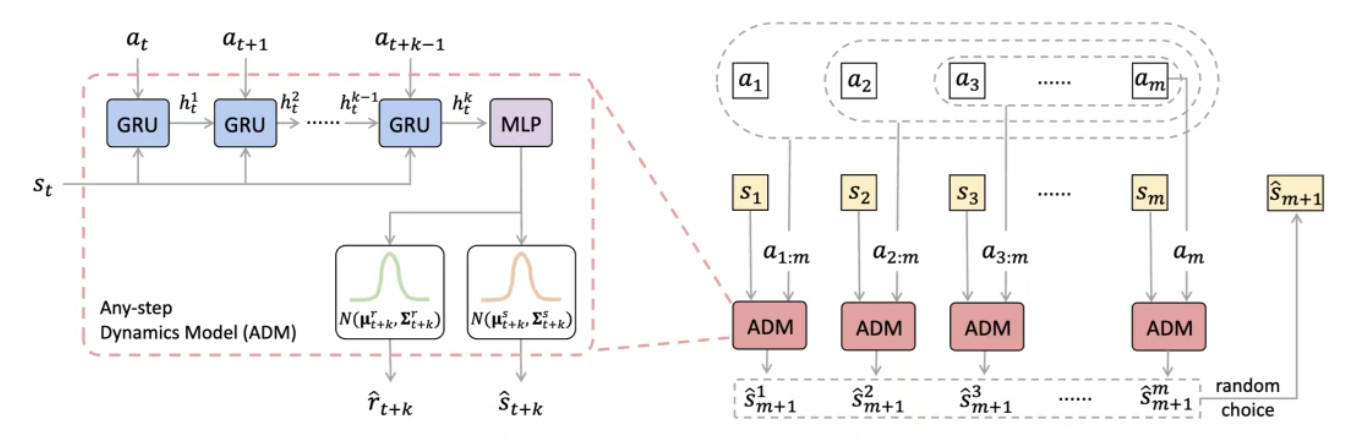
\includegraphics{images/image-0050.png}
\caption{ADM 任意步动力学模型示意图}
\end{figure}

\hypertarget{ux4e8cux6a21ux578bux67b6ux6784-3}{%
\subsubsection{（二）模型架构}\label{ux4e8cux6a21ux578bux67b6ux6784-3}}

\begin{itemize}
\tightlist
\item
  由于输入计划的步长 \(k\) 是可变的，作者采用了包含门控循环单元（GRU）的循环神经网络（RNN）来实现 ADM。
\item
  为了处理输入维度，模型会将初始的单步状态 \(s_t\) 进行复制，使其与多步动作序列的长度相匹配，然后依次送入 RNN。
\item
  RNN 输出的隐藏状态 \(h_k\) 会被送入多层感知机（MLP），最终输出目标状态 \(s_{t+k}\) 和奖励 \(r_{t+k}\) 的高斯分布参数，即均值和标准差 \((\mu_{t+k}^{s}, \Sigma_{t+k}^{s})\) 与 \((\mu_{t+k}^{r}, \Sigma_{t+k}^{r})\)。
\end{itemize}

\hypertarget{ux4e09ux8badux7ec3ux76eeux6807}{%
\subsubsection{（三）训练目标}\label{ux4e09ux8badux7ec3ux76eeux6807}}

最大化 \(k\) 步预测（\(k\) 为 \(1\) 至 \(m\) 间的任意值）的对数似然：

\[
J_T(\theta)
=
\frac{1}{m}
\sum_{k=1}^{m}
\mathbb{E}_{(s_t,a_{t:t+k-1},r_{t+k},s_{t+k}) \sim D_{\mathrm{env}}}
\left[
\log T_{\theta}^{k}(s_{t+k}, r_{t+k} \mid s_t, a_{t:t+k-1})
\right]
\]

\hypertarget{ux56dboff-policyux65f6ux7684ux4e0dux786eux5b9aux6027ux91cfux5316}{%
\subsubsection{（四）Off-policy时的不确定性量化}\label{ux56dboff-policyux65f6ux7684ux4e0dux786eux5b9aux6027ux91cfux5316}}

\begin{itemize}
\tightlist
\item
  \textbf{不确定性量化原理}：当面临轨迹分布发生变化或进入风险区域时，使用不同回溯长度 \(k\) 预测出的状态会表现出明显的分歧。ADMPO-OFF 创造性地利用这一特性，通过计算不同回溯长度 \(k\) 预测结果的方差（或标准差）来量化模型的不确定性 \(U^{\mathrm{ADM}}\)，彻底摆脱了对集成模型的依赖。
\item
  \textbf{不确定性公式}：
\end{itemize}

\[
U^{\mathrm{ADM}}(s_t, a_t)
=
\mathbb{E}_{\tau^m \sim I(\pi)}
\left[
\left\|
\frac{1}{m}
\sum_{k=1}^{m}
\left(
(\Sigma_{t}^{k})^{2}
+(\mu_t^{k})^{2}
\right)
-
(\bar{\mu})^{2}
\right\|_1
\right]
\]

\begin{itemize}
\tightlist
\item
  \textbf{悲观价值迭代机制}：在离线训练好的 ADM 中进行环境展开时，算法会对每一步生成的奖励进行惩罚：\(\tilde{r}=r-\beta U^{ADM}(s_t,a_t)\)，其中 \(\beta\) 是惩罚系数。通过惩罚高不确定性区域的奖励，算法构造了一个悲观的贝尔曼算子，强制策略保持保守，避免采取未知区域的危险动作。
\end{itemize}

\hypertarget{ux4e09adm-v2ux7684ux6539ux8fdb}{%
\subsection{三、ADM-v2的改进}\label{ux4e09adm-v2ux7684ux6539ux8fdb}}

\hypertarget{ux4e00ux72b6ux6001ux521dux59cbux5316ux4e0eux52a8ux4f5cux6f14ux5316ux5206ux79bb}{%
\subsubsection{（一）状态初始化与动作演化分离}\label{ux4e00ux72b6ux6001ux521dux59cbux5316ux4e0eux52a8ux4f5cux6f14ux5316ux5206ux79bb}}

第一代ADM通过直接建模任意步长的状态转移，减少了自举带来的误差累积。但由于其结构设计问题，ADM需要将初始状态多次复制，反复引入起始状态以对齐动作序列的长度，这导致了RNN隐藏表示与初始状态的强耦合，且无法通过并行计算加速任意步长的预测。

ADM-v2对这一结构做了更自然的重构：把状态编码和动力学预测分开，先将起始状态编码为隐变量，将这一隐表示作为循环单元的初始隐藏状态，后续递推只输入动作序列，不再重复输入起始状态。这样能让预测效果更优，也更符合基于隐变量的世界模型的范式。

\begin{figure}[htbp]
\centering
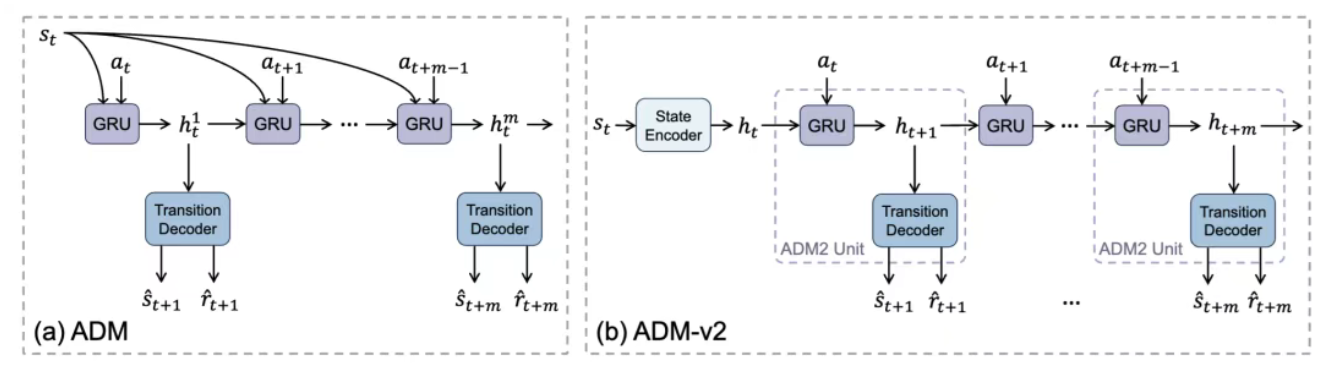
\includegraphics{images/image-0051.png}
\caption{ADM 与 ADM-v2 架构对比}
\end{figure}

模型分为三个组件：

\begin{itemize}
\tightlist
\item
  \textbf{状态编码器（State Encoder）}：将回溯起点状态 \(s_t\) 编码为隐向量 \(h_t\)，即 \(h_t=enc_{\theta}(s_t)\)。这个 \(h_t\) 直接作为 GRU 的初始隐藏状态。
\item
  \textbf{GRU 单元}：因为起点状态的信息已经压缩在 \(h_t\) 中，后续 GRU 的每次循环前向传播不再重复输入起点状态，而仅接收动作序列中的当前动作 \(a_t\)：
\end{itemize}

\[
h_{t+1}=g_{\theta}(h_t,a_t)
\]

\begin{itemize}
\tightlist
\item
  \textbf{转移解码器（Transition Decoder）}：接收更新后的隐藏状态 \(h_{t+1}\)，解码并输出下一状态 \(s_{t+1}\) 和奖励 \(r_{t+1}\) 的独立高斯分布参数：
\end{itemize}

\[
(\mu_{t+1}^{s}, \Sigma_{t+1}^{s}, \mu_{t+1}^{r}, \Sigma_{t+1}^{r})
=
\mathrm{dec}_{\theta}(h_{t+1})
\]

\hypertarget{ux4e8cux5e76ux884cux4efbux610fux6b65ux6edaux52a8ux63a8ux6f14parallel-any-step-roll-outparoll}{%
\subsubsection{（二）并行任意步滚动推演（Parallel Any-step Roll-out，PARoll）}\label{ux4e8cux5e76ux884cux4efbux610fux6b65ux6edaux52a8ux63a8ux6f14parallel-any-step-roll-outparoll}}

\begin{figure}[htbp]
\centering
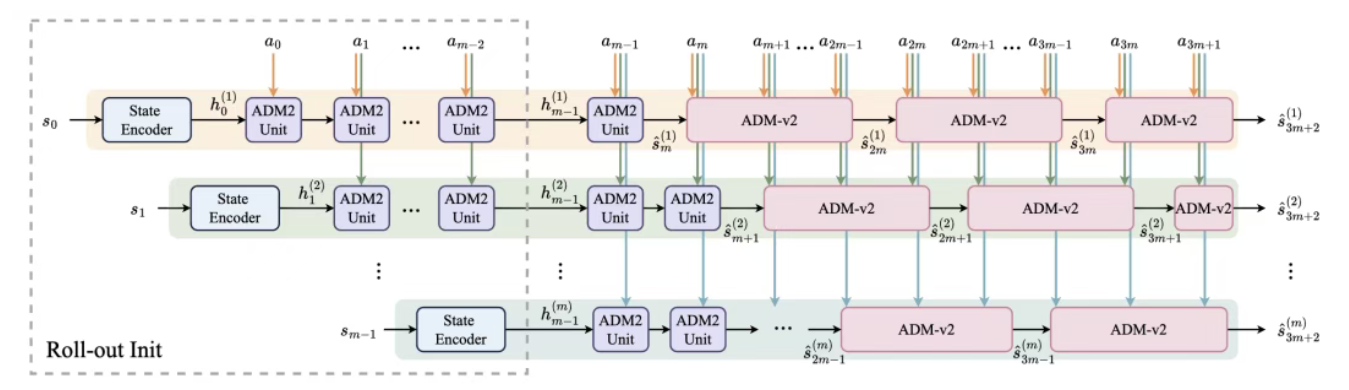
\includegraphics{images/image-0052.png}
\caption{PARoll 并行任意步滚动推演初始化示意图}
\end{figure}

如图，维护 \(m\) 个并行预测分支，每两个分支之间有 \(1\) 步的时间差，每个分支在中间都每隔 \(m\) 步（设定的最大预测步长）进行一次预测。

\textbf{第一步：轨迹初始化}

在进行模型 rollout 之前，算法首先需要构建 \(m\) 条并行的预测时间线（Timeline），其中 \(m\) 是模型训练时设定的最大预测跨度。

\begin{enumerate}
\def\labelenumi{\arabic{enumi}.}
\tightlist
\item
  \textbf{数据采样}：从真实环境离线数据集 \(D_{\mathrm{env}}\) 中采样一段长度为 \(m-1\) 的真实状态-动作序列：
\end{enumerate}

\[
(s_0,a_0,s_1,a_1,\ldots,s_{m-2},a_{m-2},s_{m-1})
\]

\begin{enumerate}
\def\labelenumi{\arabic{enumi}.}
\setcounter{enumi}{1}
\tightlist
\item
  \textbf{并行编码与对齐}：这 \(m\) 个真实状态分别作为 \(m\) 条时间线的起点。

  \begin{itemize}
  \tightlist
  \item
    第 \(1\) 条时间线以 \(s_0\) 为起点，先用状态编码器将 \(s_0\) 编码为初始隐状态 \(h_0^{(1)}\)。接着，将动作序列 \((a_0,a_1,\ldots,a_{m-2})\) 依次输入到 ADM2 Unit 中进行递归前向传播，使其时间步对齐到 \(m-1\)，最终得到隐状态 \(h_{m-1}^{(1)}\)。
  \item
    第 \(2\) 条时间线以 \(s_1\) 为起点，状态编码器将 \(s_1\) 编码为 \(h_1^{(2)}\)，然后依次输入动作 \((a_1,\ldots,a_{m-2})\) 更新隐状态，对齐到时间步 \(m-1\)，得到隐状态 \(h_{m-1}^{(2)}\)。
  \item
    依此类推，第 \(m\) 条时间线直接以 \(s_{m-1}\) 为起点，通过状态编码器编码后，直接得到时间步 \(m-1\) 的隐状态 \(h_{m-1}^{(m)}\)，无需输入任何历史动作。
  \end{itemize}
\item
  \textbf{初始化完成}：经过上述过程，我们在时间步 \(m-1\) 获得了 \(m\) 个多样化的、包含了不同历史回溯信息的隐状态集合：
\end{enumerate}

\[
(h_{m-1}^{(1)},h_{m-1}^{(2)},\ldots,h_{m-1}^{(m)})
\]

\textbf{第二步：并行生成 Roll-out 与多样化预测}

从时间步 \(t=m-1\) 开始，模型正式进入未知未来的 rollout 阶段。

\begin{enumerate}
\def\labelenumi{\arabic{enumi}.}
\tightlist
\item
  \textbf{动作采样与隐状态并行更新}：策略网络 \(\pi\) 根据当前状态给出动作 \(a_{m-1}\)。此时，\(m\) 条时间线上的 ADM2 Unit 并行接收这个动作，并同步更新各自的隐状态：
\end{enumerate}

\[
h_m^{(i)}=g_\theta(h_{m-1}^{(i)},a_{m-1})
\]

其中 \(i\in\{1,2,\ldots,m\}\) 代表不同的时间线。

\begin{enumerate}
\def\labelenumi{\arabic{enumi}.}
\setcounter{enumi}{1}
\tightlist
\item
  \textbf{状态与奖励的并行解码}：接着，转移解码器并行对这 \(m\) 个隐状态进行解码，输出预测状态和奖励的高斯分布参数，并从中采样：
\end{enumerate}

\[
(\mu_{s_m}^{(i)},\Sigma_{s_m}^{(i)},\mu_{r_m}^{(i)},\Sigma_{r_m}^{(i)})
=
dec_\theta(h_m^{(i)})
\]

\[
\hat{s}_m^{(i)}\sim\mathcal{N}(\mu_{s_m}^{(i)},\Sigma_{s_m}^{(i)}),
\quad
\hat{r}_m^{(i)}\sim\mathcal{N}(\mu_{r_m}^{(i)},\Sigma_{r_m}^{(i)})
\]

\begin{enumerate}
\def\labelenumi{\arabic{enumi}.}
\setcounter{enumi}{2}
\item
  \textbf{预测多样性的来源}：在同一时间步 \(m\) 预测出的 \(m\) 个状态 \((\hat{s}_m^{(1)},\hat{s}_m^{(2)},\ldots,\hat{s}_m^{(m)})\) 具有天然的多样性，因为它们来自不同的回溯起点和不同长度的跨度（Stride）直接预测而来。例如，\(\hat{s}_m^{(1)}\) 是从 \(s_0\) 经过 \(m\) 步动作演化而来，而 \(\hat{s}_m^{(m)}\) 是从 \(s_{m-1}\) 经过 \(1\) 步动作演化而来。
\item
  \textbf{持续演化}：对于后续的时间步 \(t\gt m\)，算法重复执行并行的隐状态更新和解码生成操作。在此过程中，从 \(m\) 个多样化预测中均匀随机选择一个作为下一步策略采样的依据，并同时利用这些预测的方差来并行估计当前步的模型不确定性 \(U^{ADM2}\)。
\end{enumerate}

\textbf{模型不确定性估计}：在每一步 \(t\)，算法从上述 \(m\) 个多样化预测中均匀选取一个作为下一步的真实采样，并利用不同时间线的分布方差来量化模型在该处的不确定性（Model Uncertainty, \(U^{ADM2}\)）：

\[
U^{\mathrm{ADM2}}(s_t,a_t)
=
\mathbb{E}
\left[
\left\|
\frac{1}{m}
\sum_{k=1}^{m}
\left(
(\Sigma_{s_t}^{(k)})^2
+
(\mu_{s_t}^{(k)})^2
\right)
-
(\bar{\mu}_t)^2
\right\|_1
\right]
\]

\textbf{第三步：跨度重置}

由于 ADM-v2 在训练时设定了最大预测跨度为 \(m\)，多步直接预测（即隐状态的连续传播）不能无限期地进行下去，否则会导致严重的误差累积。

\begin{enumerate}
\def\labelenumi{\arabic{enumi}.}
\item
  \textbf{重置触发条件}：当某条时间线的直接预测步数达到最大跨度 \(m\) 时，必须截断隐状态的传播，并进行重置（Reset）。
\item
  \textbf{重置方法}：调用状态编码器（State Encoder），将该时间线在当前时间节点刚刚预测出的状态重新编码，作为新的起始隐状态送入下一个长度为 \(m\) 的预测窗口。例如，对于第 \(i\) 条时间线，它的重置时间节点是 \((m+i-1,2m+i-1,3m+i-1,\ldots)\)，此时隐状态更新方式变为：
\end{enumerate}

\[
h_{m+i-1}^{(i)}=\mathrm{enc}_\theta(\hat{s}_{m+i-1}^{(i)})
\]

\begin{enumerate}
\def\labelenumi{\arabic{enumi}.}
\setcounter{enumi}{2}
\tightlist
\item
  \textbf{交错重置的高效性}：在图中可以清晰地看到，不同时间线的重置操作（图中右侧断开的箭头并重新引入 ADM-v2 块的起点）在时间轴上是交错排列的（呈对角线状）。在实际执行时，每个时间步仅有一条时间线（具体为 \((t\bmod m)+2\)）会达到最大跨度并触发重置。这意味着每一步只需要执行一次额外的状态编码器前向传播，极大地保证了算法的运行效率。
\end{enumerate}

这意味着每隔 \(m\) 步就要把隐状态输出为预测状态，以此重新编码新的隐状态，完成重置。这样相比于随机回溯步数的好处在于，无论随机选中哪一条分支，都能获得来自历史较远状态和较近状态的信息（每隔 \(m\) 步一个状态），更好地满足平衡防止误差累积和提高精度的需要。

\hypertarget{ux56dbux5168ux89c6ux91cerolloutux7684ux7406ux8bbaux8fb9ux754c}{%
\subsubsection{（四）全视野rollout的理论边界}\label{ux56dbux5168ux89c6ux91cerolloutux7684ux7406ux8bbaux8fb9ux754c}}

\begin{enumerate}
\def\labelenumi{\arabic{enumi}.}
\tightlist
\item
  \textbf{离线策略优化：ADM2PO-fh}
\end{enumerate}

在离线学习中，策略极易陷入动力学模型预测不准确（即不确定性高）的未来系数区域（Out-of-distribution）。ADM-v2 利用 PARoll 估计的不确定性 \(U^{ADM2}\) 作为悲观惩罚项（Penalty term）。

\begin{itemize}
\tightlist
\item
  \textbf{定理 3.1（不确定性量化器有效性）}：论文证明了 \(\beta\cdot U^{\mathrm{ADM2}}\) 是一个合法的 \(\epsilon\)-不确定性量化器。它严格界定了真实 Bellman 算子与 ADM-v2 代理算子之间的误差上界：
\end{itemize}

\[
\left|
\hat{T}^{\pi}Q(s_t,a_t)
-
T^{\pi}Q(s_t,a_t)
\right|
\le
\beta\cdot U^{\mathrm{ADM2}}(s_t,a_t)
\]

\begin{itemize}
\tightlist
\item
  \textbf{应用}：基于此，ADM2PO-fh 算法在 \(Q\) 值估计中引入修正项：
\end{itemize}

\[
\hat{T}^{\mathrm{ADM2}}Q(s_t,a_t)
:=
\hat{T}^{\pi}Q(s_t,a_t)
-
\beta\cdot U^{\mathrm{ADM2}}(s_t,a_t)
\]

从而在面临高风险区域时收紧 \(Q\) 值，防止过估计。

\begin{enumerate}
\def\labelenumi{\arabic{enumi}.}
\setcounter{enumi}{1}
\tightlist
\item
  \textbf{离线策略评估（OPE）：ADM2OPE}
\end{enumerate}

ADM-v2 可以直接作为一个 surrogate environment（代理环境），通过让待评估的策略在模型中进行 \(N\) 次完整的全视野轨迹采样，取平均回报作为策略的评估值。

\begin{itemize}
\tightlist
\item
  \textbf{定理 3.2（性能边界 Bounds）}：评估回报与真实回报的差距受限于长期预测误差和策略散度。论文证明了返回的差距受到 \(C(\delta_{\max},\epsilon_r)\) 的约束：
\end{itemize}

\[
\left|
\eta(\pi)-\hat{\eta}(\pi)
\right|
\le
\frac{2\gamma r_{\max}\delta_{\max}}{(1-\gamma)(1-\gamma^m)}
+
\frac{2\gamma r_{\max}\epsilon_\pi}{(1-\gamma)^2}
+
\frac{4r_{\max}\epsilon_r}{1-\gamma}
\]

\begin{itemize}
\tightlist
\item
  \textbf{核心结论}：当最大 \(m\) 步直接预测误差满足特定条件（\(\delta_{\max}\lt\frac{\delta(1-\gamma^m)}{1-\gamma}\)）时，ADM-v2 生成的 OPE 误差上界比传统的单步动力学模型更加紧致（Tighter），理论上提供了更可靠的评估。
\end{itemize}

\hypertarget{ux53c2ux8003ux6587ux732e-190}{%
\subsection{参考文献}\label{ux53c2ux8003ux6587ux732e-190}}

\begin{itemize}
\tightlist
\item
  Lin, H., Xu, Y.-Y., Sun, Y., Zhang, Z., Li, Y.-C., Jia, C., Ye, J., Zhang, J., \& Yu, Y. (2025). \href{https://openreview.net/forum?id=JZCxlrwjZ8}{Any-step Dynamics Model Improves Future Predictions for Online and Offline Reinforcement Learning}. ICLR.
\item
  Lin, H., Xiao, S., Li, Y.-C., Zhang, Z., Sun, Y., Jia, C., \& Yu, Y. (2026). \href{https://openreview.net/forum?id=ICbXEwqpga}{ADM-v2: Pursuing Full-Horizon Roll-out in Dynamics Models for Offline Policy Learning and Evaluation}. ICLR.
\end{itemize}

\clearpage

\hypertarget{action-spaceux7684ux5b66ux4e60ux8bbaux6587}{%
\section{Action Space的学习（论文）}\label{action-spaceux7684ux5b66ux4e60ux8bbaux6587}}

\begin{quote}
本文是论文阅读笔记，内容代表对应论文方法或作者理解，不应直接视为领域共识或工程最佳实践。
\end{quote}

\hypertarget{ux4e00latent-action-models}{%
\subsection{一、Latent Action Models}\label{ux4e00latent-action-models}}

世界模型的核心表达式是 \(s_{t+1}=f(s_t,a_t)\)。对于海量的视频数据，\(s_t\) 和 \(s_{t+1}\) 都是容易获取的，但我们却没有显式的动作数据 \(a_t\)。这会影响模型学习``特定干预会造成何种后果''，尤其是在交互式或具身智能场景中更明显。如果将动作看作一种模态，那么模型也需要一个对应的``词表''，即 Action Space。Latent Action Models 是一种从视频中自监督学习 Action Space 的方法。

\hypertarget{ux4e00ux6838ux5fc3ux7ec4ux4ef6}{%
\subsubsection{（一）核心组件}\label{ux4e00ux6838ux5fc3ux7ec4ux4ef6}}

\begin{enumerate}
\def\labelenumi{\arabic{enumi}.}
\tightlist
\item
  反向动力学模型（Inverse Dynamics Model）：从前后状态 \(s_t\) 和 \(s_{t+1}\) 中推断动作 \(a_t\) 的潜在表示，并通过信息瓶颈促使 \(a_t\) 编码最关键的运动信息。
\item
  前向动力学模型（Forward Dynamics Model）：使用当前状态 \(s_t\) 和动作 \(a_t\) 预测下一状态 \(s_{t+1}\)。
\end{enumerate}

\hypertarget{ux4e8cux62bdux8c61ux8981ux6c42}{%
\subsubsection{（二）抽象要求}\label{ux4e8cux62bdux8c61ux8981ux6c42}}

如果允许动作 \(a_t\) 保留太多信息以提升生成质量，它又容易混入颜色、纹理、背景等内容信息，导致动作不够抽象、难以迁移。为了保证动作表示具有可迁移性和抽象性，模型通常会施加强预测瓶颈，例如向量量化或变分瓶颈。

但不可否认的是，如果动作表示被压缩得足够抽象，它更容易迁移，却也可能偏离动作空间内在的流形结构，丢失预测下一个状态的准确性，以及生成所需的细节。

\hypertarget{ux4e8cux52a8ux4f5cux62bdux8c61ux5316ux4e2dux7684ux7ed3ux6784-ux5185ux5bb9ux8868ux5f81ux89e3ux8026ux65b9ux6cd5}{%
\subsection{二、动作抽象化中的结构-内容表征解耦方法}\label{ux4e8cux52a8ux4f5cux62bdux8c61ux5316ux4e2dux7684ux7ed3ux6784-ux5185ux5bb9ux8868ux5f81ux89e3ux8026ux65b9ux6cd5}}

\hypertarget{ux4e00ux6838ux5fc3ux601dux60f3-25}{%
\subsubsection{（一）核心思想}\label{ux4e00ux6838ux5fc3ux601dux60f3-25}}

前面提到，对于 Latent Action Models 提取动作，一方面需要施加信息瓶颈以保证动作的抽象性；另一方面，如果压缩过度又会影响预测准确性。对于这一对矛盾，论文《DiLA: Disentangled Latent Action World Models》提出了结构-内容解耦的方法：将时空变换结构与视觉内容的表征解耦，在动作（即状态随时空变换的结构）上采取严格的信息瓶颈，在视觉内容方面则通过额外通道避免信息丢失。

\hypertarget{ux4e8cux6a21ux578bux67b6ux6784ux4e0eux5de5ux4f5cux6d41-1}{%
\subsubsection{（二）模型架构与工作流}\label{ux4e8cux6a21ux578bux67b6ux6784ux4e0eux5de5ux4f5cux6d41-1}}

输入视频先经过 DINOv2 编码器和 Spatial-Temporal Transformer，得到视觉表征。随后，模型将这些表征分别送入不同通路中处理：

\begin{enumerate}
\def\labelenumi{\arabic{enumi}.}
\tightlist
\item
  结构通路：负责建模与运动相关的空间结构，例如位置、布局和动态变化。模型先压缩得到结构表征，再用逆向动力学模型从连续结构表征的差异中推断动作的潜在表示。前向动力学模型根据当前结构表征和动作预测下一时刻的结构表征。这个过程使动作表征主要编码``结构如何变化''，而不是完整图像如何变化。
\item
  内容通路：负责保存视觉细节，例如颜色、纹理、背景、物体外观和历史信息。模型使用线性注意力 Mamba 层作为记忆模块，用于聚合历史内容信息。它关注相对稳定的视觉内容，而不是快速变化的动态结构。
\end{enumerate}

最后，Fusion Decoder 将预测出的结构表征、内容记忆表征以及初始帧信息融合起来，重建未来视觉表征。

\begin{figure}[htbp]
\centering
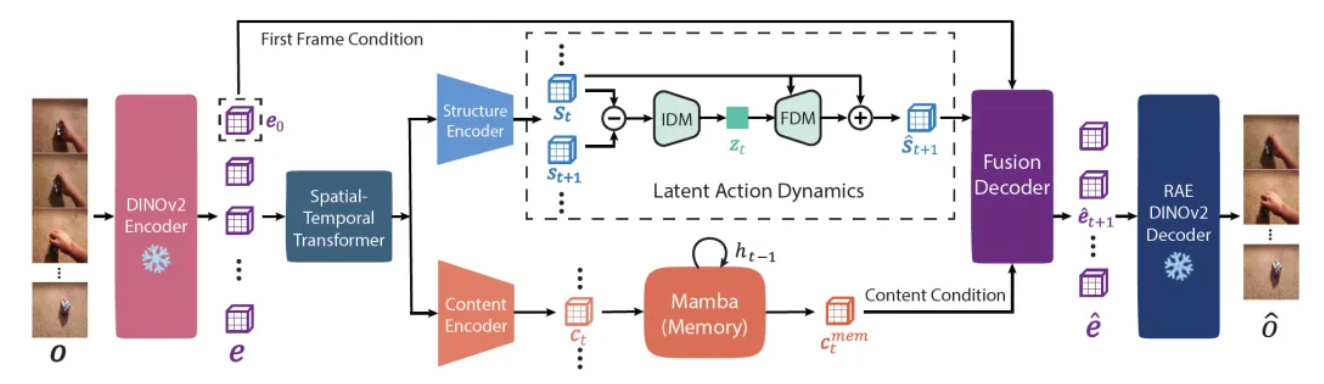
\includegraphics{images/image-0053.png}
\caption{DiLA 动作空间学习模型架构}
\end{figure}

为了验证结构与内容是否真正分离，论文设计了实验：从一个视频中提取结构，从另一个视频中提取内容，然后将二者重新组合生成新序列。生成序列继承了结构序列的空间动态，同时保留了内容序列的颜色、纹理和外观属性。而固定结构表征，只让内容的记忆模块随时间更新，序列保持静止。这说明内容记忆模块主要编码时间上相对稳定的内容信息，而不是运动本身。

\hypertarget{ux53c2ux8003ux6587ux732e-191}{%
\subsection{参考文献}\label{ux53c2ux8003ux6587ux732e-191}}

\begin{itemize}
\tightlist
\item
  Schmidt, D., \& Jiang, M. (2024). \href{https://openreview.net/forum?id=rnnt2Be6nN}{Learning to Act without Actions}. International Conference on Learning Representations.
\item
  Garrido, Q., Nagarajan, T., Terver, B., Ballas, N., LeCun, Y., \& Rabbat, M. (2026). \href{https://arxiv.org/abs/2601.05230}{Learning Latent Action World Models In The Wild}. arXiv:2601.05230.
\end{itemize}

\clearpage
